\documentclass[a4paper,12pt,twoside]{article}

\usepackage[ngerman,english]{babel}

%%% FOR DISPLAYING CODE
\usepackage[procnames]{listings}
\usepackage{xcolor}

%%% MARGINS
\usepackage{geometry}
% INFO: https://www.overleaf.com/learn/latex/Page_size_and_margins
\geometry{
	a4paper,
%	total={170mm,257mm},
	left=25mm,
	top=25mm,
	textwidth=16cm,
	textheight=23cm,
%	right=25mm,
%	bottom=40mm,$
}

%%% SPACING
%\usepackage{setspace} 
%\onehalfspacing

\usepackage{siunitx} % for writing numbers with units % e.g. \SI{6.3e8}{km}, \ang{62.59}, \num{100}'s \si{km}, \SI{53}{\degree}
\usepackage{amsmath,amssymb}
\usepackage{graphicx}
\usepackage{datetime} 
\usepackage{color}
\usepackage{float} %without it, tables position more or less random, with this an writing \begin{table}[H] the table appears right where it is defined!
\usepackage{mathptmx}
\usepackage{enumitem}

\usepackage[T1]{fontenc}
\usepackage[utf8]{inputenc}

\usepackage{pgfplots} % for plotting functions
\pgfplotsset{compat=1.16}

%%% HEADER and FOOTER
%\usepackage[automark,headsepline]{scrpage2}
%\ihead[]{\headmark}
%\chead[]{}
%\ohead[]{\pagemark}
%\ifoot[]{}
%\cfoot[\pagemark]{}
%\ofoot[]{}
%\pagestyle{scrheadings}

\usepackage{lipsum}

%% LINE SPACING
\usepackage{setspace}
\setstretch{1.5}

%%% HYPERLINKS
\usepackage{hyperref} % muss sich vor cite stuff befinden

%% SET IMAGE PATH (where images are stored)
\graphicspath{{figures/}}

%%% CITE
\usepackage{apacite}
\bibliographystyle{apacite}

%%%%%%%%%%%%%%%%%%%%%%%%%%%%%%%%%%
% DEFINE COLORS
\definecolor{red}{rgb}{0.6,0,0} 
\definecolor{blue}{rgb}{0,0,0.6}
\definecolor{green}{rgb}{0,0.8,0}
\definecolor{cyan}{rgb}{0.0,0.6,0.6}

\definecolor{mypink}{rgb}{0.753,0.000,0.890}
\definecolor{myblue}{rgb}{0.078,0.000,1.000}
\definecolor{mybluedark}{rgb}{0.004,0.024,0.525} \definecolor{mygreen}{rgb}{0.000,0.514,0.000}
\definecolor{myreddark}{rgb}{0.698,0.000,0.008}
\definecolor{mycyan}{rgb}{0.000,0.506,0.612}
\definecolor{mybrown}{rgb}{0.494,0.365,0.090}

%%% DISPLAY CODE
\usepackage{listings}
\newcommand\pythonstyle{\lstset{
    language=Python,
	tabsize=4,
	basicstyle=\normalsize\sffamily,
	numberstyle=\color{gray},
	stringstyle=\color{myreddark},
    commentstyle=\color{mygreen},
    % KEYWORDS
    % main keywords
	keywordstyle=\normalsize\color{myblue},%\bfseries,
    % add keywords (main blue)
    emph={False,None,True,self,TODO},
    emphstyle={\color{myblue}},
    % pink emph
    emph={[2]assert,break,continue,del,elif ,else,except,finally,for,from,global,if,import,in,pass,raise,return,try,while,with,yield},
    emphstyle={[2]\color{mypink}},%\bfseries,
    %dark blue emph
    emph={[3]execfile,reduce,xrange},
    emphstyle={[3]\color{mybluedark}},
    % brown emph
    emph={[4]exec,print,isinstance,zip,enumerate,reversed,len,repr},
    emphstyle={[4]\color{mybrown}},
    % cyan emph
    emph={[5]object,type,list,set,dict,tuple,str,super},
    emphstyle={[5]\color{mycyan}},
    % errors (also cyan emph)
    emph={[6]Exception,NameError,IndexError,SyntaxError,TypeError,ValueError,OverflowError,ZeroDivisionError},
    emphstyle={[6]\color{mycyan}},
    % errors (also cyan emph)
    emph={[7]copy,deepcopy,append,real,imag},
    emphstyle={[7]\color{black}},
    % 
    showstringspaces=false,
	breaklines=true,
	numbers=left,
    frame=tb,
	xleftmargin=15pt
}}

\newcommand\javascriptstyle{\lstset{
	basicstyle=\small\sffamily,
    keywordstyle=\color{blue}\bfseries,
    commentstyle=\color{purple}\ttfamily,
    stringstyle=\color{red}\ttfamily,
	numberstyle=\color{gray},
    keywords={typeof, new, true, false, catch, function, return, null, catch, switch, var, if, in, while, do, else, case, break},
    ndkeywords={class, export, boolean, throw, implements, import, this},
    ndkeywordstyle=\color{darkgray}\bfseries,
    identifierstyle=\color{black},
    comment=[l]{//},
    morecomment=[s]{/*}{*/},
    morestring=[b]',
    morestring=[b]",
    showstringspaces=false,
	breaklines=true,
	numbers=left,
    frame=tb,
	xleftmargin=15pt,
    sensitive=false,
}}

\newcommand\csharpstyle{\lstset{
	language=csh,
	tabsize=4,
	basicstyle=\small\sffamily,
	numberstyle=\color{gray},
	stringstyle=\color{myreddark},
    commentstyle=\color{mygreen},
	morecomment=[l]{//}, %use comment-line-style!
	morecomment=[s]{/*}{*/}, %for multiline comments
    % KEYWORDS
	keywordstyle=\normalsize\color{myblue},%\bfseries,
	morekeywords={ abstract, event, new, struct,
		as, explicit, null, switch,
		base, extern, object, this,
		bool, false, operator, throw,
		break, finally, out, true,
		byte, fixed, override, try,
		case, float, params, typeof,
		catch, for, private, uint,
		char, foreach, protected, ulong,
		checked, goto, public, unchecked,
		class, if, readonly, unsafe,
		const, implicit, ref, ushort,
		continue, in, return, using,
		decimal, int, sbyte, virtual,
		default, interface, sealed, volatile,
		delegate, internal, short, void,
		do, is, sizeof, while,
		double, lock, stackalloc,
		else, long, static,
		enum, namespace, string},
	% 
    showstringspaces=false,
	breaklines=true,
	numbers=left,
    frame=tb,
	xleftmargin=15pt	
}}

% Python environment
\lstnewenvironment{python}[1][]
{
	\pythonstyle
	\lstset{#1}
}
{}
\lstnewenvironment{javascript}[1][]
{
	\javascriptstyle
	\lstset{#1}
}
{}
\lstnewenvironment{csharp}[1][]
{
	\csharpstyle
	\lstset{#1}
}
{}

% CODE FOR EXTERNAL FILES
\newcommand\pythonexternal[2][]{{
		\pythonstyle
		\lstinputlisting[#1]{#2}}}

% CODE FOR INLINE
\newcommand\pythoninline[1]{{\pythonstyle\lstinline!#1!}}
\newcommand\csharpinline[1]{{\csharpstyle\lstinline!#1!}}
\newcommand\javascriptinline[1]{{\javascriptstyle\lstinline!#1!}}

%% DEFINE CUSTOM COMMANDS AND SHORTCUTS

% some commands
\def\ba#1\ea{\begin{align}#1\end{align}}
\def\bas#1\eas{\begin{align*}#1\end{align*}}
\def\bmat#1\emat{\begin{pmatrix}#1\end{pmatrix}}
\newcommand{\ve}[1]{\vec{#1}}
\newcommand{\veTwo}[2]{\begin{pmatrix}#1\\#2\end{pmatrix}}
\newcommand{\veThree}[3]{\begin{pmatrix}#1\\#2\\#3\end{pmatrix}}
\newcommand{\veFour}[4]{\begin{pmatrix}#1\\#2\\#3\\#4\end{pmatrix}}
\newcommand{\ora}[1]{\overrightarrow{#1}}
\newcommand{\ola}[1]{\overleftarrow{#1}}
\newcommand{\s}[1]{\sqrt{#1}}

\def \bit{\begin{itemize}\setlength\itemsep{0em}} %\vspace{-5mm}
	\def \eit{\end{itemize}}

\def \ben{\begin{enumerate}\setlength\itemsep{0em}} %\vspace{-5mm}
	\def \een{\end{enumerate}}

\def \N{\mathbb{N}}
\def \Z{\mathbb{Z}}
\def \Q{\mathbb{Q}}
\def \R{\mathbb{R}}
\def \C{\mathbb{C}}

\def \ra{\rightarrow}
\def \longra{\longrightarrow}
\def \Ra{\Rightarrow}
\def \Longra{\Longrightarrow}
\def \la{\leftarrow}
\def \longla{\longleftarrow}
\def \La{\Leftarrow}
\def \Longla{\Longleftarrow}

\def \lra{\leftrightarrow}
\def \longlra{\longleftrightarrow}
\def \Lra{\Leftrightarrow}
\def \Longlra{\Longleftrightarrow}

\def \l{\left}
\def \r{\right}

\def \a{\alpha}
\def \b{\beta}
\def \g{\gamma}

\def \c{\cdot}

\def \el{\in}
\def \notel{\notin}

\newcommand{\f}{\frac}

\def \q{\quad}
\newcommand{\p}{\phantom}

\def\bs#1\es{\begin{split}#1\end{split}}


\def \L{\mathbb{L}}




\begin{document}

%%%%%%%%%%%%%%%%%%%%%%%%%%%%%%%%%%%%%%%%%%%%%%%%%%%%%%%
%%%%%%%%%%%%%%%%%%%%%%%%%%%%%%%%%%%%%%%%%%%%%%%%%%%%%%%
%%%%%%%%%%%%%%%%%%%%%%%%%%%%%%%%%%%%%%%%%%%%%%%%%%%%%%%

%%% AB HIER ARBEITEN, WEITER OBEN NICHTS VERAENDERN
%%% Ausnahme: Einbinden weitere Pakete

\selectlanguage{ngerman} %% HIER SPRACHE EINSTELLEN! english, ngerman

\begin{titlepage}
	\clearpage\thispagestyle{empty}	
	\setstretch{1}
	
	\begin{minipage}[t]{\textwidth}
		\begin{minipage}[t]{0.5\textwidth}
			Zeynep Zülal Keskin\\
			Mattfeldstrasse 6\\
			9532 Rickenbach b. Wil\\
			077 277 43 77\\
			zekeskin@ksr.ch
		\end{minipage}
		\begin{minipage}[t]{0.5\textwidth}
			\begin{flushright}
				Kantonsschule Romanshorn\\
				Klasse 4Ma\\
				Maturaarbeit
			\end{flushright}
		\end{minipage}
	\end{minipage}
	
	\vspace{4cm}
	{
		\centering
		\Huge\bfseries Simulationen des N-Körper-Problems mit dem Barnes-Hut-Algorithmus \par
		\vspace{1cm}
		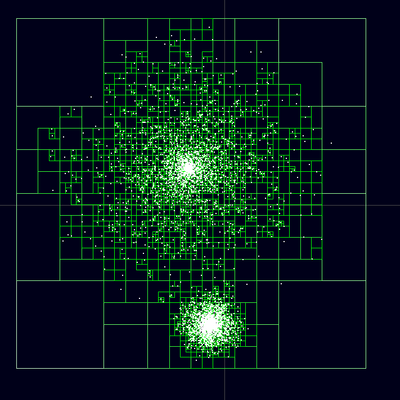
\includegraphics[width=0.15\textwidth]{Barnes_hut_tree.png}\par
	}
	
	\vspace{9cm}	
	\noindent
    Fach: Physik \noindent\\
	Betreuungsperson: Dr. Andreas Schärer\\
	Abgabetermin: 6. Januar 2025
	
\end{titlepage}

%%%%%%%%%%%%%%%%%%%%%%%%%%%%%%%%%%%%%%%%%%%%%%%%%%%%%%%
%%%%%%%%%%%%%%%%%%%%%%%%%%%%%%%%%%%%%%%%%%%%%%%%%%%%%%%
%%%%%%%%%%%%%%%%%%%%%%%%%%%%%%%%%%%%%%%%%%%%%%%%%%%%%%%

% \null\thispagestyle{empty}\clearpage

%%% ABSTRACT

\pagenumbering{roman}

\section*{Abstract}

Das N-Körper-Problem ist ein fundamentales Problem der Himmelsmechanik, 
das die Bewegung von N Massenpunkten unter gegenseitiger gravitativer Anziehung beschreibt. 
Diese Arbeit untersucht zwei verschiedene Simulationsmethoden für das N-Körper-Problem: 
die direkte Methode und den Barnes-Hut-Algorithmus. Ziel ist es, die Genauigkeit und 
Effizienz dieser Methoden zu analysieren und zu vergleichen.
%%%%%%%%%%%%%%%%%%%%%%%%%%%%%%%%%%%%%%%%%%%%%%%%%%%%%%%
%%%%%%%%%%%%%%%%%%%%%%%%%%%%%%%%%%%%%%%%%%%%%%%%%%%%%%%
%%%%%%%%%%%%%%%%%%%%%%%%%%%%%%%%%%%%%%%%%%%%%%%%%%%%%%%

%%% TABLE OF CONTENTS

%\null\thispagestyle{empty}\clearpage
\newpage
%\setcounter{page}{1}
\tableofcontents

\parindent=0pt
\parskip=6pt

\newpage

\pagenumbering{arabic}

%%%%%%%%%%%%%%%%%%%%%%%%%%%%%%%%%%%%%%%%%%%%%%%%%%%%%%%
%%%%%%%%%%%%%%%%%%%%%%%%%%%%%%%%%%%%%%%%%%%%%%%%%%%%%%%
%%%%%%%%%%%%%%%%%%%%%%%%%%%%%%%%%%%%%%%%%%%%%%%%%%%%%%%

\section{Einleitung}
Diese Arbeit befasst sich mit einem der grundlegendsten und komplexesten Probleme der Himmelsmechanik und -dynamik: 
dem N-Körper-Problem in der Physik. Dieses Problem ist nicht nur von theoretischem Interesse, 
sondern findet auch praktische Anwendungen in der Astronomie, Raumfahrt und vielen anderen Bereichen der Physik. 
Die zentrale Forschungsfrage dieser Arbeit lautet: Welche mathematischen und physikalischen Methoden können verwendet werden, 
um die Bewegung von N-Körpern zu beschreiben und zu verstehen? 
Das Ziel dieser Arbeit ist es, die Bewegung von N-Körpern zu definieren und umfassend zu analysieren. 
Dabei soll der physikalische Hintergrund dieses Problems beleuchtet und seine historische Entwicklung nachgezeichnet werden. 
Ein besonderer Schwerpunkt liegt auf der Darstellung und Untersuchung der verschiedenen mathematischen und physikalischen Methoden, 
die im Laufe der Zeit entwickelt wurden, um die Dynamik von N-Körpern zu erklären.
Darüber hinaus werden zwei detaillierte Simulationen entwickelt, um die theoretischen Konzepte praktisch zu veranschaulichen. 
Diese Simulationen dienen nicht nur der Erklärung des Problems, sondern auch dem Vergleich verschiedener Lösungsansätze. 
Durch diese Herangehensweise soll ein tieferes Verständnis für die Komplexität des N-Körper-Problems und die Herausforderungen bei seiner Lösung vermittelt werden.
Ein weiterer Aspekt dieser Arbeit ist die Untersuchung der praktischen Relevanz des N-Körper-Problems. 
Dabei wird aufgezeigt, wie die theoretischen Erkenntnisse in der Astronomie zur Berechnung von Planetenbahnen, 
in der Raumfahrt zur Planung von Satellitenmissionen und in anderen Bereichen der Physik zur Modellierung komplexer Systeme angewendet werden können.
Zusammenfassend strebt diese Arbeit an, einen umfassenden Überblick über das N-Körper-Problem zu geben, seine Bedeutung 
in der modernen Physik aufzuzeigen und durch die Entwicklung und den Vergleich von Simulationen einen Beitrag zur Lösung 
dieses faszinierenden und herausfordernden Problems zu leisten.
\newpage


\section{Theoretische Grundlagen}

\subsection{Problembeschreibung und historische Entwicklung}
Das N-Körper-Problem beschäftigt sich mit der dynamischen Analyse von N Massepunkten, die durch ihre gegenseitige gravitative Anziehung beeinflusst werden. Während das Zwei-Körper-Problem durch Newtons Gesetz der universellen Gravitation und die Keplerschen Gesetze exakt gelöst werden kann, wird das N-Körper-Problem für N Körper wesentlich komplexer und zeigt in der Regel chaotisches Verhalten. Die historische Entwicklung dieses Problems begann im 17. Jahrhundert mit den grundlegenden Arbeiten von Johannes Kepler und Isaac Newton, die die Basis für die Himmelsmechanik schufen. Im 18. und 19. Jahrhundert erweiterten Joseph-Louis Lagrange und Pierre-Simon Laplace das Verständnis durch die Einführung der Lagrangeschen Gleichungen und durch die Analyse spezieller Lösungen wie der Lagrange-Punkte, die besondere Gleichgewichtslagen in einem gravitativen System beschreiben. Henri Poincaré entdeckte Ende des 19. Jahrhunderts die chaotische Natur des Systems, was den Beginn der modernen Chaosforschung einleitete. Im 20. und 21. Jahrhundert ermöglichten Fortschritte in der Computertechnologie und numerischen Methoden präzise Simulationen und Analysen komplexer N-Körper-Systeme, die wichtige Einblicke in die Dynamik von Galaxien und die Planung von Raumfahrtmissionen bieten.

\subsection{Gravitationskraft}
Die Gravitationskraft $\vec{F}_{12}$ zwischen zwei punktförmigen Massen $m_1$ und $m_2$ liegt auf der Verbindungslinie der beiden Massen.
Der Betrag $F$ der Gravitationskraft ist proportional zu den Massen $m_1$ und $m_2$ sowie umgekehrt proportional zum Quadrat des Abstands $r$ 
(die relative Position ist die Position eines Körpers relativ zu einem anderen: \(\vec{r} = \vec{r}_2 - \vec{r}_1\)) der Massen~\cite{LeifiPhysikGravitation}. Er berechnet sich durch:
\begin{align*}
	F = G \frac{m_1 m_2}{r^2}
\end{align*}
mit der Gravitationskonstante $G = \SI{6.674e-11}{\frac{m^3}{kg\,s^2}}$.

\subsection{Die Keplerschen Gesetze}
Die Keplerschen Gesetze beschreiben die Bewegung von Planeten um die Sonne und sind grundlegende Prinzipien der Himmelsmechanik. Johannes Kepler formulierte sie im frühen 17. Jahrhundert auf Basis der Beobachtungen von Tycho Brahe. Diese Gesetze markierten einen Wendepunkt von der klassischen, kreisförmigen Vorstellung der Planetenbewegung zu einem elliptischen Modell. Im Folgenden werde ich die drei Keplerschen Gesetze erläutern~\cite{LeifiPhysikKepler}.
\subsubsection{1. Keplersches Gesetz: Das Gesetz der Ellipsen}
Das erste Keplersche Gesetz besagt:
\begin{quote}
    Die Bahnen der Planeten um die Sonne sind Ellipsen, wobei sich die Sonne in einem der beiden Brennpunkte befindet.
\end{quote}
Mathematisch lässt sich eine Ellipse durch die Gleichung
\begin{align*}
	\frac{x^2}{a^2} + \frac{y^2}{b^2} = 1
\end{align*}

beschreiben, wobei \(a\) die grosse Halbachse und \(b\) die kleine Halbachse der Ellipse ist. Der Planet bewegt sich auf einer solchen Ellipsenbahn, wobei sich die Sonne nicht im Zentrum der Ellipse befindet, sondern in einem der beiden Brennpunkte. Dies war ein entscheidender Unterschied zur zuvor angenommenen Kreisbahn der Planeten.
\subsubsection{2. Keplersches Gesetz: Das Gesetz der Flächen}
Das zweite Keplersche Gesetz lautet:

\begin{quote}
    Der Fahrstrahl (die Verbindungslinie) zwischen einem Planeten und der Sonne überstreicht in gleichen Zeitspannen gleiche Flächen.
\end{quote}
Dies bedeutet, dass sich ein Planet auf seiner elliptischen Bahn unterschiedlich schnell bewegt: Er ist schneller, wenn er sich näher an der Sonne befindet (Perihel) und langsamer, wenn er weiter entfernt ist (Aphel). Dies lässt sich mathematisch durch die Erhaltung des Drehimpulses ausdrücken, da der Winkelgeschwindigkeitsvektor und der Abstand zur Sonne in Beziehung stehen. Formal lässt sich dies auch durch die Flächengeschwindigkeit beschreiben:
\begin{align*}
	\frac{dA}{dt} = \text{konstant},
\end{align*}

wobei \(A\) die Fläche und \(t\) die Zeit ist. Diese Konstanz der Flächengeschwindigkeit ist ein Hinweis auf das Prinzip der Erhaltung des Drehimpulses.

\subsubsection{3. Keplersches Gesetz: Das Harmoniegesetz}
Das dritte Keplersche Gesetz beschreibt die Beziehung zwischen der Umlaufzeit eines Planeten und seiner Entfernung von der Sonne:
\begin{quote}
    Die Quadrate der Umlaufzeiten zweier Planeten verhalten sich wie die Kuben der großen Halbachsen ihrer Bahnen.
\end{quote}
Mathematisch wird dies durch die Gleichung
\begin{align*}
	\frac{T_1^2}{T_2^2} = \frac{a_1^3}{a_2^3}
\end{align*}

ausgedrückt, wobei \(T_1\) und \(T_2\) die Umlaufzeiten der beiden Planeten und \(a_1\) und \(a_2\) die grossen Halbachsen ihrer Bahnen sind. Dies zeigt, dass Planeten, die weiter von der Sonne entfernt sind, eine längere Umlaufzeit haben als solche, die sich näher an der Sonne befinden~\cite{Haase1998}.

\subsection{Zwei-Körper-Problem}
Das 2-Körper-Problem ist ein zentrales Modell der Himmelsmechanik, das die Bewegung zweier Massen untersucht, die sich unter dem Einfluss ihrer gegenseitigen Gravitation befinden. Es beschreibt ein isoliertes System, in dem keine äusseren Kräfte wirken, und ermöglicht die analytische Bestimmung der Bahnen, auf denen sich die Körper bewegen~\cite{Spektrum}. Diese Bahnen, die je nach Anfangsbedingungen elliptisch, parabolisch oder hyperbolisch sein können, liefern wichtige Erkenntnisse über die Dynamik von Planeten, Monden und Satelliten. Als analytisch lösbares Problem bildet es die Grundlage für die Erweiterung auf komplexere Mehrkörpersysteme und spielt eine wesentliche Rolle in der Astronomie und Physik.

\subsubsection{Die Mathematische Beschreibung}

Da sich die beiden Körper (Massen \( m_1, m_2 \), Positionen \( \vec{x_1}, \vec{x_2} \)) ausschliesslich gegenseitig beeinflussen, lauten die Bewegungsgleichungen:

\begin{align*}
	m_1 \ddot{\vec{x}}_1 &= \vec{F}_{1,2} \\
	m_2 \ddot{\vec{x}}_2 &= \vec{F}_{2,1}
\end{align*}

Die Kräfte \( \vec{F}_{1,2} und \vec{F}_{2,1} \) hängen gemäss dem Relativitätsprinzip nur von der relativen Position der Körper zueinander ab. Der Vektor \( \vec{r} := \vec{x_1} - \vec{x_2} \) 
beschreibt die Position des zweiten Körpers relativ zum ersten, während der Vektor \( \vec{R} \) den Ortsvektor des Schwerpunkts oder Baryzentrums des Systems darstellt. 
Darüber hinaus sind die beiden Kräfte nach dem 3. Newtonschen Axiom einander entgegengesetzt und gleich gross:

\begin{align*}
\vec{F}_{1,2} = -\vec{F}_{2,1} = \vec{F}(\vec{r})
\end{align*}

\subsubsection{Übergang zum äquivalenten Einkörperproblem}
Die mathematische Modellierung der Position zweier Körper im Raum basiert auf Positionsvektoren, die vom Koordinatenursprung ausgehen. Dabei erfolgt die Berechnung in Relativ- und Schwerpunktkoordinaten siehe Abb.\ref{Zwei-Körper}.

\begin{figure}[H]
	\centering
	\includegraphics[width=0.4\textwidth]{Zwei-Körper.png}
	\caption[Eintrag in Abbildungsverzeichnis von der Mathematische Modellierung der Zwei Körper]{Mathematische Modellierung der Lage zweier Körper im Raum, x1 und x2 sind vom Koordinatenursprung ausgehende Positionsvektoren.}
	\label{Zwei-Körper}
\end{figure}

\begin{align*}
	\vec{r} &= \vec{x_1} - \vec{x_2} \\
	\vec{R} &= \frac{m_1 \vec{x_1} + m_2 \vec{x_2}}{M} \quad (M = m_1 + m_2 \text{ ist die Gesamtmasse.})
\end{align*}

Durch die Addition geeigneter Vielfacher der beiden oben genannten Bewegungsgleichungen lassen sich zwei voneinander unabhängige Bewegungsgleichungen ableiten:

\begin{align*}
	\ddot{\vec{R}} &= 0 \\
	\vec{r} &= \left( \frac{1}{m_1} + \frac{1}{m_2} \right) \vec{F}_{1,2}
\end{align*}

Die erste Gleichung zeigt, dass der Massenschwerpunkt eine geradlinige und gleichförmige Bewegung ausführt, was auch dem allgemeinen Schwerpunktsatz entspricht. Die zweite Gleichung kann entsprechend umgeformt werden zu:

\begin{align*}
\mu \ddot{\vec{r}} = \vec{F}(\vec{r}),
\end{align*}

wobei,

\begin{align*}
\mu = \left( \frac{1}{m_1} + \frac{1}{m_2} \right)^{-1} = \frac{m_1 m_2}{M}
\end{align*}
Die reduzierte Masse des Zweikörperproblems wird als $\mu$ bezeichnet. Sie ist stets kleiner als die kleinere der beiden Massen und nähert sich dieser an, wenn die grössere Masse gegen unendlich geht. Die zugehörige Bewegungsgleichung beschreibt, dass die Relativkoordinate $\vec{r}(t)$ sich so verhält, als ob ein Körper der Masse $\mu$ sich in einem ortsfesten Kraftfeld $\vec{F}(\vec{r})$ bewegt wird. Dies entspricht dem äquivalenten Einkörperproblem. Für alle Fälle, in denen die Stärke der Kraft von einer Potenz des Abstandes $r$ abhängt, wurde es zuerst von Newton gelöst~\cite{Gleisner2013}.

\subsubsection{Gemeinsame Bewegung}
Nachdem das Einkörperproblem durch die Bahnkurve $\vec{r}(t)$
gelöst wurde und die Bewegung des Schwerpunktes $\vec{R}(t)$
ebenfalls bekannt ist, lässt sich das System wieder in die ursprünglichen Koordinaten zurücktransformieren:

\begin{align*}
	\vec{x_1}(t) &= \vec{R}(t) + \frac{m_2}{M} \vec{r}(t) \\
	\vec{x_2}(t) &= \vec{R}(t) - \frac{m_1}{M} \vec{r}(t)
\end{align*}

Wird das System im Schwerpunkt betrachtet (mathematisch, durch eine Koordinatentransformation, insbesondere eine Verschiebung um \( \vec{R} \) anwendet), so bewegen sich beide Körper um den Schwerpunkt, der stets auf ihrer Verbindungsline liegt und beschreibt zwei zur Kurve \( \mathbf{r}(t) \) ähnliche Bahnen, deren Grössenverhältnis durch das reziproke Massenverhältnis bestimmt ist. Durch zweimaliges Differenzieren von \( \vec{x_1}(t) \) und Einsetzen von

\begin{align*}
	\vec{r} = \frac{M}{m_2} \vec{x_1}
\end{align*}

Man erkennt, dass für den ersten Körper die Bewegungsgleichung laute

\begin{align*}
	m_1 \ddot{\vec{x}}_1 = \vec{F}_{\text{eff}}(\vec{x_1})
\end{align*}

erfüllt ist, sodass der Körper sich in einem effektiven Kraftfeld:

\begin{align*}
	\vec{F}_{\text{eff}}(\vec{x_1}) = \vec{F} \left( \frac{M}{m_2} \vec{x_1} \right)
\end{align*}

bewegen würde. Das Zentrum dieses Kraftfeldes bleibt ortsfest am Schwerpunkt, und seine Stärke entspricht dem realen Kraftfeld, jedoch in einer durch das Massenverhältnis bestimmten größeren Entfernung - dasselbe gilt auch für den anderen Körper.
Wenn sich der Schwerpunkt geradlinig und gleichförmig bewegt und weitere geeignete Anfangsbedingungen erfüllt sind, beschreiben die Bahnen der beiden Körper eine Art „Schlangenkurve“ um die Bahn des Schwerpunktes.
In der Astronomie ermöglicht diese sogenannte Taumelbewegung die indirekte Beobachtung unsichtbarer Begleiter von Sternen, wie beispielsweise Exoplaneten.

\subsubsection{Drehimpulserhaltung}

Die Kraft \( \vec{F}_{1,2} = -\vec{F}_{2,1} = \vec{F}(\vec{r}) \) verläuft parallel zur Verbindungsline \( \vec{r} \) (entsprechend der Problemdefinition). Daher handelt es sich um eine Zentralkraft, die kein Drehmoment auf den umlaufenden Körper ausübt, da dieses durch das Vektorprodukt von Radiusvektor und Kraft bestimmt wird:

\begin{align*}
	\vec{r} \times \vec{F} = 0
\end{align*}

Daher bleibt der Drehimpuls \( \vec{L} = \vec{r} \times \vec{p} \) hinsichtlich Betrag und Richtung zeitlich konstant. Er stellt ein Bewegungsintegral dar. Dies bedeutet, dass die Bewegung in einer festen Ebene erfolgt, da die Vektoren \( \vec{r} \) und \( \vec{p} = \mu \vec{r} \) stets in der zur \( \vec{L} \) senkrechten Ebene liegen.
Aus der Konstanz des Drehimpulses folgt zudem das 2. Keplersche Gesetz, auch bekannt als Flächensatz, das für jedes Zentralkraftfeld gilt. In ebenen Polarkoordinaten zerfällt die vektorielle Bewegungsgleichung des Einkörperproblems schließlich in zwei gekoppelte gewöhnliche Differentialgleichungen:

\begin{align*}
	\dot{r} - r \dot{\varphi}^2 = - \frac{1}{\mu} F(r) \\
	\frac{d}{dt} \left( \mu r^2 \dot{\varphi} \right) = 0
\end{align*}
Die zweite dieser Gleichungen bestätigt erneut die Erhaltung des Drehimpulses \( L \), denn:

\begin{align*}
	L = \mu r^2 \dot{\varphi}
\end{align*}

\subsubsection{Energieerhaltung}
Für das Keplerproblem im engeren Sinne wird die Kraft durch die Gravitation beschrieben:

\begin{align*}
	F(r) = - \frac{G m_1 m_2}{r^2}
\end{align*}
Wendet man die Definition des Drehimpulses in Polarkoordinaten an, um die Winkelgeschwindigkeit \( \dot{\varphi} \) aus der anderen Differentialgleichung zu eliminieren, so erhält man eine Gleichung für den Abstand \( r \), die Radialgleichung:

\begin{align*}
	\mu \ddot{r} = \frac{L^2}{\mu r^3} - \frac{G M}{r^2}
\end{align*}

Durch Multiplikation mit \( \dot{r} \) und \( \mu \) lässt sich diese Gleichung auch in der Form schreiben:

\begin{align*}
	\frac{d}{dt} \left( \frac{\mu}{2} \dot{r}^2 + \frac{L^2}{2 \mu r^2} - \frac{GM \mu}{r} \right) = 0
\end{align*}

Die Terme in dieser Gleichung entsprechen dem radialen Anteil der kinetischen Energie, dem winkelabhängigen Anteil der kinetischen Energie, der als Zentrifugalpotential die Radialbewegung beeinflusst, sowie der potenziellen Energie des Körpers im äusseren Zentralpotential. Zusammen ergeben sie die Gesamtenergie~\cite{Physik-Schule}:

\begin{align*}
	E = \frac{\mu}{2} \dot{r}^2 + \frac{L^2}{2 \mu r^2} - \frac{GM \mu}{r}
\end{align*}
Diese Gesamtenergie bleibt laut der obigen Gleichung zeitlich konstant und ist somit ebenfalls ein Bewegungsintegral. Die Erhaltung der Gesamtenergie folgt direkt daraus, dass es sich bei einem Gravitationsfeld um ein konservatives Feld handelt. Weiterführende Informationen zu diesem Thema finden sich im Artikel zur spezifischen Bahnenenergie, der diese Zusammenhänge detaillierter behandelt.

\subsubsection{Bahnkurve-Kegelschnittform}

Gibt man die Werte für die beiden Integrale der Bewegung \( E \) und \( L \) vor, so lässt sich die Bewegungsgleichung lösen, indem man zunächst die radiale Bewegung \( r(t) \) aus der Form des Energieintegrals (letzte Gleichung im obigen Abschnitt) und anschliessend die Winkelbewegung \( \varphi(t) \) aus dem Drehimpulsintegral \( L = \mu r^2 \dot{\varphi} \) berechnet. 
Allerdings führt dieser Ansatz auf Gleichungen, die als unanschaulich gelten, da man ihnen die Form der Bahn nicht direkt entnehmen kann. 
Daher ist es üblich, entweder die Radialgleichung oder das Energieintegral zunächst in eine Differentialgleichung nach dem Winkel \( \varphi \) umzuwandeln. Dabei wird \( r \) als Funktion von \( \varphi \) betrachtet und die Ableitung \( r' := \frac{dr}{d\varphi} \) nach dem Winkel \( \varphi \) eingeführt. 
Hier wird der zweite Weg vorgestellt, bei dem das Energieintegral verwendet wird. 
Mit der Energiegleichung aus dem vorigen Abschnitt und indem man \( \dot{r} \) durch \( r' \dot{\varphi} \) und \( \dot{\varphi} \) mit Hilfe der Drehimpulsgleichung durch \( \frac{L}{\mu r^2} \) ersetzt, erhält man so:

\begin{align*}
	E = \frac{L^2}{2\mu r^2} \left( \frac{r^2}{r^2 + 1} \right) - \frac{GM\mu}{r}
\end{align*}
Die Bahnkurve, die diese Gleichung löst, ist, wenn man die Willkür in der Wahl des Winkels \( \varphi \) so ausnutzt, dass der größte oder kleinste Abstand vom Zentrum bei \( \varphi = 0 \) liegt, von der Form

\begin{align*}
	r(\varphi) = \frac{p}{1 + \epsilon \cos \varphi}
\end{align*}
wobei man durch Einsetzen nachrechnen kann, dass für die beiden Parameter

\begin{align*}
	p = \frac{L^2}{GM\mu^2} \quad \text{und} \quad \epsilon^2 = \frac{2E L^2}{GM^2 \mu^2} + 1
\end{align*}

gelten muss. Dies ist die Gleichung eines Kegelschnitts mit numerischer Exzentrizität \( \epsilon \) (wobei \( \epsilon \geq 0 \) gewählt werden kann, denn der Wechsel \( \epsilon \to -\epsilon \) ist äquivalent zu \( \varphi \to \varphi + \pi \)).
Ist die Gesamtenergie negativ, dann gilt \( \epsilon < 1 \) und die Bewegung ist gebunden, d. h., es gibt einen maximalen Abstand (Aphelion) \( \frac{p}{1 - \epsilon} \) vom Zentrum. Es handelt sich bei der Bahn in diesem Fall um eine Ellipse, in deren einem Brennpunkt das Zentrum liegt, deren große Halbachse

\begin{align*}
	a = \frac{p}{1 - \epsilon^2}
\end{align*}
ist. Dies ist das erste keplersche Gesetz (der Ellipsensatz). Dass die Bahnkurve des gebundenen Zustands immer geschlossen ist, ist bei radialsymmetrischen Kraftfeldern ein Spezialfall, der sonst nur noch beim harmonischen Oszillator vorkommt, dessen Kraftfeld proportional zum Abstand vom Zentrum wächst.
Ist die Gesamtenergie positiv, so ist \( \epsilon > 1 \) und die Bahn ist eine Hyperbel mit kleinstem Abstand \( \frac{p}{1 + \epsilon} \) vom Zentrum. Der Grenzfall mit Energie \( E = 0 \) und \( \epsilon = 1 \) ist eine Parabel, deren kleinster Abstand vom Zentrum \( \frac{p}{2} \) ist~\cite{Krug2011}.

In einem idealisierten Zwei-Körper-Problem, bei dem nur die gegenseitige Gravitationskraft wirkt und keine anderen Störungen oder relativistischen Effekte berücksichtigt werden, bewegen sich die Körper immer entlang einer Kegelschnittbahn (Ellipse, Parabel oder Hyperbel).
\begin{figure}[H]
	\centering
	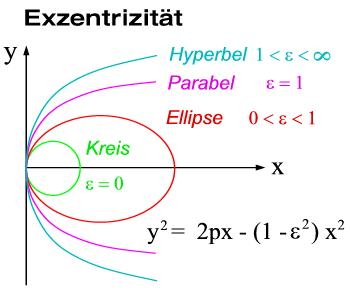
\includegraphics[width=0.4\textwidth]{exzentrizitaet.jpg}
	\caption[Eintrag in Abbildungsverzeichnis von Kegelschnittbahnen]{Kegelschnittbahnen}
	\label{Exzentrizität}
\end{figure}

\subsection{Drei-Körper-Problem}
Im Gegensatz zum Zwei-Körper-Problem, das durch die Kepler-Gesetze vollständig analytisch lösbar ist, gibt es für das Drei-Körper-Problem keine allgemeine analytische Lösung. Das Problem beschreibt die Bewegung dreier Körper (z.\,B.\ Sterne, Planeten oder Monde), die sich gegenseitig aufgrund der Gravitation anziehen. Jeder Körper wird durch die resultierende Gravitationskraft der beiden anderen beeinflusst, was zu einer sehr komplizierten Dynamik führt.
Für das Zwei-Körper-Problem kann die Bewegung der beiden Körper auf elliptische, parabolische oder hyperbolische Bahnen reduziert werden, je nach den Anfangsbedingungen. Das Drei-Körper-Problem hingegen führt oft zu unvorhersehbaren, chaotischen Bewegungen, außer in speziellen Fällen mit symmetrischen oder stark eingeschränkten Anfangsbedingungen.

\subsubsection{Mathematische Beschreibung}
Das Drei-Körper-Problem befasst sich mit der Bestimmung der Bewegung von drei Massen \( m_1 \), \( m_2 \) und \( m_3 \), die durch ihre wechselseitigen Gravitationskräfte miteinander interagieren. Die Beschleunigung jeder dieser Körper wird durch die Gravitationsanziehung der beiden anderen Massen bestimmt, gemäß dem Gravitationsgesetz von Newton. Die Position jedes Körpers wird durch seinen Vektor \( \mathbf{r}_i \) im dreidimensionalen Raum beschrieben. Die Gravitationskraft zwischen zwei Körpern nimmt mit der dritten Potenz des Abstands zwischen ihnen ab, wobei die resultierende Kraft auf jeden Körper die Summe der von den beiden anderen Körpern ausgeübten Kräfte ist. Dies führt zu einem System gekoppelter, nichtlinearer Differentialgleichungen, bei dem die Beschleunigung jedes Körpers von den relativen Positionen aller drei Massen abhängt. Aufgrund der Komplexität dieses Systems ist eine exakte analytische Lösung im Allgemeinen nicht möglich, weshalb es in der Regel numerisch gelöst wird.
Die wichtigsten Gleichungen, die die Bewegung der drei Körper beschreiben, sind:
\begin{align*}
	\ddot{\vec{r}}_1 = -G m_2 \frac{\vec{r}_1 - \vec{r}_2}{|\vec{r}_1 - \vec{r}_2|^3} - G m_3 \frac{\vec{r}_1 - \vec{r}_3}{|\vec{r}_1 - \vec{r}_3|^3} \\
	\ddot{\vec{r}}_2 = -G m_3 \frac{\vec{r}_2 - \vec{r}_3}{|\vec{r}_2 - \vec{r}_3|^3} - G m_1 \frac{\vec{r}_2 - \vec{r}_1}{|\vec{r}_2 - \vec{r}_1|^3} \\
	\ddot{\vec{r}}_3 = -G m_1 \frac{\vec{r}_3 - \vec{r}_1}{|\vec{r}_3 - \vec{r}_1|^3} - G m_2 \frac{\vec{r}_3 - \vec{r}_2}{|\vec{r}_3 - \vec{r}_2|^3}
\end{align*}


Diese Gleichungen beschreiben, wie sich die Beschleunigungen der drei Körper aufgrund ihrer gegenseitigen Gravitationskräfte entwickeln~\cite{threebodylibretexts}.

\subsubsection{Bekannte Lösungen des Dreikörperproblems}
\paragraph{1- Klassische Bahnen:}
Das System, das die Bewegung von drei gravitativ wechselwirkenden Körpern beschreibt, 
kann im Allgemeinen nicht analytisch gelöst werden. 
Es existieren jedoch zwei bekannte analytische Lösungen, 
die auf Euler und Lagrange zurückgehen.
Bei der Euler-Bahn beginnen die drei Körper in einer kollinearen Anordnung. 
Die beiden äusseren Körper bewegen sich auf einem Kreis um den zentralen Körper, 
der sich im Mittelpunkt dieses Kreises befindet (siehe Abb.\ref{EulerUndLagrange} 2a).
Bei der Lagrange-Bahn starten die drei Körper an den Eckpunkten eines gleichseitigen 
Dreiecks. Während der Bewegung behalten sie diese dreieckige Struktur bei und 
bewegen sich gemeinsam auf einem Kreis (siehe Abb.\ref{EulerUndLagrange} 2b)~\cite{Ramos2019}.

\begin{figure}[H]
	\centering
	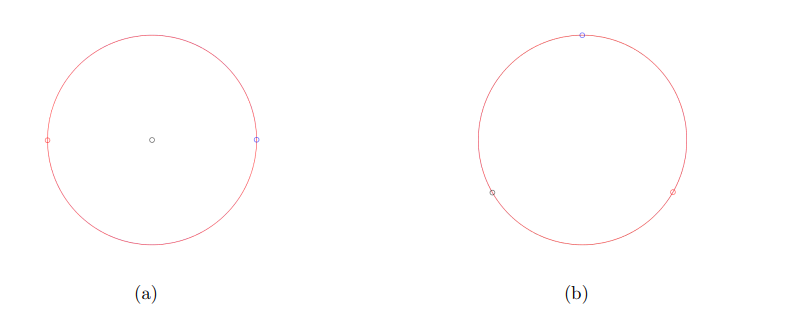
\includegraphics[width=0.8\textwidth]{EulerUndLagrange.png}
	\caption[Eintrag in Abbildungsverzeichnis von Euler und Lagrange Orbit]{Klassische Drei-Körper-Orbits: (a) Euler-Orbit, (b) Lagrange-Orbit.}
	\label{EulerUndLagrange}
\end{figure}

\paragraph{2- Figure-8:}
Die Figure-Eight-Bahn ist eine spezielle, periodische Lösung des 
Drei-Körper-Problems in der Himmelsmechanik. 
Drei Massenpunkte gleicher Masse bewegen sich dabei entlang 
einer symmetrischen Bahn in Form einer Acht. 
Diese Lösung wurde 1993 von Christopher Moore entdeckt und 
später von Carles Simó analysiert. 
Sie zeichnet sich durch Null-Drehimpuls und 
eine perfekte Balance der Gravitationskräfte aus, 
wodurch die Bewegung stabil bleibt. Die Bahn ist ein seltenes 
Beispiel für geordnete Dynamik in einem ansonsten chaotischen System und 
bietet wertvolle Einblicke in die Theorie der Mehrkörperprobleme.
\begin{figure}[H]
    \centering
    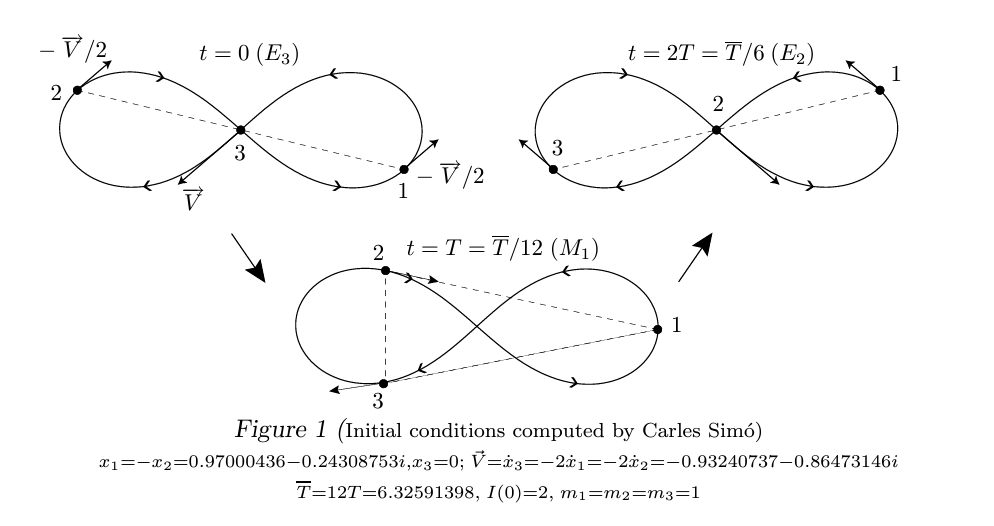
\includegraphics[width=0.7\textwidth]{figure8.png}
    \caption[Eintrag in Abbildungsverzeichnis von Figure-8]{Figure-8}
    \label{figure8}
\end{figure}


\paragraph{3- Das Eingeschränkte Drei-Körper-Problem:}
Das eingeschränkte Drei-Körper-Problem ist ein Spezialfall der klassischen Mechanik, bei dem die Bewegung eines dritten Körpers mit vernachlässigbarer Masse - wie eines Satelliten - unter dem gravitativen Einfluss zweier massereicher Primärkörper untersucht wird. Diese bewegen sich auf stabilen, kreisförmigen Bahnen um ihren gemeinsamen Schwerpunkt.
Das Modell setzt voraus, dass die Masse des dritten Körpers die Bewegung der Primärkörper nicht beeinflusst und dass alle drei Körper in derselben Ebene liegen. Es dient der Vereinfachung komplexer dynamischer Systeme und zur Analyse von Gleichgewichtspunkten.
Ein zentraler Anwendungsbereich ist die Berechnung von Satellitenbahnen im Erde-Mond- oder Sonne-Erde-System, insbesondere die Untersuchung der Lagrange-Punkte, an denen sich die Gravitationskräfte und die Zentrifugalkraft ausgleichen. Hier kann der dritte Körper eine stabile Position einnehmen~\cite{Weber}.

\subsubsection{Integration Methoden}
Zur Lösung des Systems von gewöhnlichen Differentialgleichungen (DGL), das die Bewegung der Körper beschreibt, ist der Einsatz eines numerischen Solvers erforderlich, um eine approximative Lösung zu erhalten. Es existiert eine Vielzahl von Solvern, die je nach ihrer Genauigkeit (Ordnung) sowie den spezifischen Eigenschaften, die sie aufweisen, ausgewählt werden können.

\paragraph{4.1 Euler-Verfahren: }
Dies ist der einfachste numerische DGL-Solver. Für ein System, das in Vektorschreibweise als $ \dot{y} = f(t, y) $, und mit einem Zeitschritt $\delta t$, geschrieben wird, wird der Wert von $y$ zum Zeitpunkt $t + \delta t$, $y_{i+1}$, in Bezug auf den Wert von $y$ zum Zeitpunkt $t$, $y_i$, berechnet als~\cite{Zhou&Long2018}:
\begin{equation*}
    y_{i+1} = y_i + f(t, y_i)\delta t
\end{equation*}
Dies ist ein Verfahren erster Ordnung, d.h. der Fehler in der Näherung ist von der Ordnung $\delta t$. Dies macht das Verfahren sehr ungenau, und es ist notwendig, einen sehr kleinen Zeitschritt anzugeben, um eine gute Näherung zu erhalten.

\paragraph{Runge-Kutta-Verfahren vierter Ordnung}
Das Runge-Kutta-Verfahren vierter Ordnung (rk4-Verfahren) ist eine Erweiterung des Euler-Verfahrens, das die Genauigkeit verbessert, indem mehr Auswertungen des Systems pro Schritt vorgenommen werden. Für ein System, das in Vektorschreibweise als $\dot{y} = f(t, y)$ und mit einem Zeitschritt $\delta t$ geschrieben wird, wird der Wert von $y$ zum Zeitpunkt $t + \delta t$, $y_{i+1}$, in Bezug auf den Wert von $y$ zum Zeitpunkt $t$, $y_i$, berechnet als:

\begin{align*}
    k_1 &= f(t, y_i)\delta t \\
    k_2 &= f\left(t + \frac{\delta t}{2}, y_i + \frac{k_1}{2} \delta t \right) \delta t \\
    k_3 &= f\left(t + \frac{\delta t}{2}, y_i + \frac{k_2}{2} \delta t \right) \delta t \\
    k_4 &= f(t + \delta t, y_i + k_3 \delta t) \delta t \\
    y_{i+1} &= y_i + \frac{1}{6}(k_1 + 2k_2 + 2k_3 + k_4)
\end{align*}

Dies ist ein Verfahren vierter Ordnung, d.h., der Fehler in der Näherung hat die Ordnung $(\delta t)^4$. Dies macht das Verfahren deutlich genauer als das Euler-Verfahren. Zum Vergleich mit dem Euler-Verfahren müssen wir denselben Zeitschritt $\delta t$ wählen, aber viermal so viele Auswertungen pro Zeitschritt vornehmen, da das rk4-Verfahren viermal so viele Auswertungen des Systems pro Zeitschritt erfordert~\cite{Swarthmore2005}.

\subsection{N-Körper Problem}
Das n-Körper-Problem ist ein klassisches Problem in der Physik und beschreibt die Bewegung mehrerer Massenpunkte, die sich gegenseitig durch ihre Gravitationskräfte beeinflussen. Die Grundgleichung für die Beschleunigung eines Körpers \( j \) in einem solchen System ist gegeben durch:

\begin{align*}
	m_j \ddot{\vec{r}}_j = G \sum_{\substack{k=1 \\ k \neq j}}^n \frac{m_j m_k (\vec{r}_k - \vec{r}_j)}{|\vec{r}_k - \vec{r}_j|^3}
\end{align*}

Hier steht \( m_j \) für die Masse des betrachteten Körpers, \( \vec{r}_j \) für dessen Position, und \( G \) für die Gravitationskonstante. Die Summe erstreckt sich über alle anderen Körper \( k \) (mit \( k \neq j \)), die eine Gravitationskraft auf den Körper \( j \) ausüben. Der Ausdruck \( \frac{\vec{r}_k - \vec{r}_j}{|\vec{r}_k - \vec{r}_j|^3} \) beschreibt dabei die Richtung und Stärke der Gravitationskraft zwischen den beiden Körpern \( j \) und \( k \), wobei der Abstand \( |\vec{r}_k - \vec{r}_j| \) hoch drei im Nenner steht, um sicherzustellen, dass die Kraft gemäss dem Gravitationsgesetz mit dem Quadrat des Abstands abnimmt~\cite{Schäfer2017}.

Das n-Körper-Problem stellt eine Herausforderung dar, weil ab mehr als zwei Körpern eine chaotische Dynamik entsteht, die eine exakte analytische Lösung unmöglich macht. Während das Zwei-Körper-Problem stabile, vorhersagbare Bahnen liefert, wird das System bei drei oder mehr Körpern extrem empfindlich gegenüber Anfangsbedingungen.
Dadurch sind die Bewegungen der Körper langfristig unvorhersehbar und schwer exakt zu berechnen. Numerische Simulationen, die die Bewegung der Körper Schritt für Schritt berechnen, bieten eine Lösungsmöglichkeit, jedoch nur in Form von Näherungen. Die Berechnungen sind dabei extrem aufwendig, da für jede Wechselwirkung die Kräfte separat berücksichtigt werden müssen, was bei steigender Körperanzahl exponentiell mehr Rechenleistung erfordert.


\section{Material und Methoden}

\subsection{Der Barnes-Hut-Algorithmus}
Der Barnes-Hut-Algorithmus ist ein effizientes Näherungsverfahren zur Berechnung der Kräfte in N-Körper-Problemen, insbesondere in der Astrophysik. Er wurde 1986 von Josh Barnes und Piet Hut entwickelt und reduziert den Rechenaufwand von $O(N^2)$ auf $O(N \log N)$, wodurch Simulationen mit einer großen Anzahl von Teilchen ermöglicht werden.
Der Algorithmus basiert auf der Annahme, dass Gruppen von weit entfernten Teilchen als einzelne Massepunkte behandelt werden können. Dazu wird der Raum rekursiv in immer kleinere Bereiche unterteilt, bis jeder Bereich entweder leer ist oder genau ein Teilchen enthält. Diese Struktur wird in Form eines Baumes, genauer eines Quadtrees im zweidimensionalen Raum oder eines Octrees im dreidimensionalen Raum, dargestellt.

\subsubsection{Algorithmusschritte}

\paragraph{1. Baumerstellung:}
Der gesamte Raum wird in vier (2D) bzw. acht (3D) Quadranten unterteilt. Jedes Teilchen wird entsprechend seiner Position in einen dieser Quadranten einsortiert. Ist ein Quadrant bereits belegt, wird er weiter unterteilt, bis jedes Teilchen in einem eigenen Unterquadranten liegt. Dieses rekursive Unterteilen führt zur Bildung des Quadtrees bzw. Octrees~\cite{Wu2024}.

\begin{figure}[H]
	\centering
	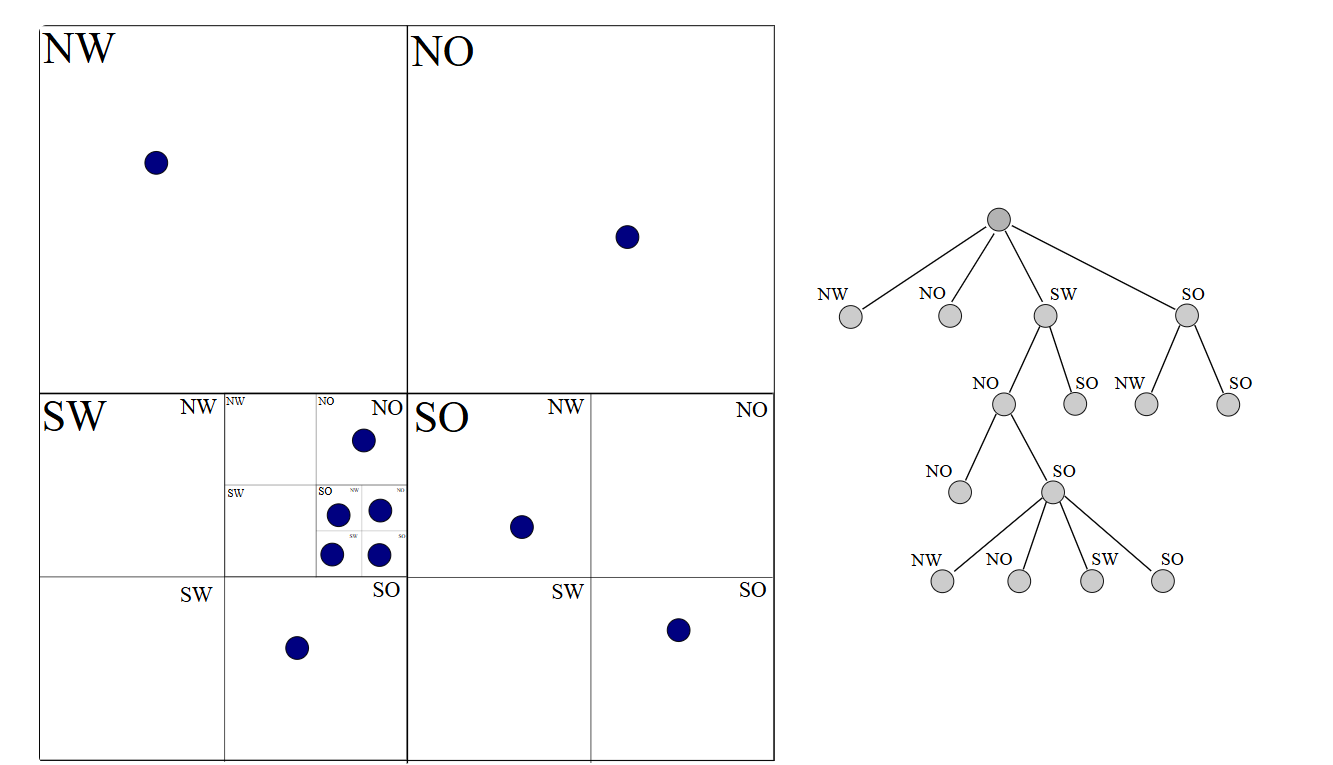
\includegraphics[width=0.8\textwidth]{Baumstruktur.png}
	\caption[Eintrag in Abbildungsverzeichnis von Baumstruktur]{Baumstruktur}
	\label{Baumstruktur}
\end{figure}

\paragraph{2. Masseverteilung:}
Nach der Baumerstellung wird für jeden Knoten des Baumes die Gesamtmasse und der Massenschwerpunkt der in ihm enthaltenen Teilchen berechnet~\cite{Burtscher&Pingali2011}. Diese Informationen sind entscheidend für die spätere Kraftberechnung.

\paragraph{3. Kraftberechnung:}
Um die auf ein bestimmtes Teilchen wirkende Kraft zu berechnen, wird der Baum erneut durchlaufen. Für jeden Knoten wird das Verhältnis von dessen Grösse zur Entfernung zum betrachteten Teilchen berechnet~\cite{BarnesHutBeltoforion}. Ist dieses Verhältnis kleiner als ein vorgegebener Schwellenwert ($\theta$), wird der gesamte Knoten als eine einzelne Masse im Massenschwerpunkt betrachtet. Andernfalls werden die Unterknoten weiter untersucht. Dieses Verfahren reduziert die Anzahl der notwendigen Kraftberechnungen erheblich.

\subsubsection{Parameter $\theta$}
Der Schwellenwert $\theta$ bestimmt die Genauigkeit der Näherung. Ein kleiner Wert für $\theta$ führt zu einer höheren Genauigkeit, da weniger Gruppierungen vorgenommen werden und mehr direkte Berechnungen stattfinden. Ein grösserer Wert reduziert den Rechenaufwand, kann jedoch die Genauigkeit beeinträchtigen. Typischerweise wird $\theta$ auf Werte um 0.5 bis 1 gesetzt, abhängig von den Anforderungen an die Simulation.

\subsubsection{Vorteile und Anwendungen}
Der Barnes-Hut-Algorithmus ermöglicht die Simulation von Systemen mit Millionen von Teilchen, was mit direkten Berechnungsmethoden unpraktikabel wäre. Er findet Anwendung in der Astrophysik, beispielsweise bei der Simulation von Galaxien, sowie in anderen Bereichen wie der Molekulardynamik und der Informatik, etwa beim kräftebasierten Zeichnen von Graphen~\cite{Heer2017}.

\subsection{React.js - Funktionsweise und Anwendungen}

React.js ist eine JavaScript-Bibliothek, die zur Entwicklung 
von Benutzeroberflächen verwendet wird. 
Sie basiert auf einer komponentenbasierten Architektur, 
bei der Anwendungen in wiederverwendbare, eigenständige 
Komponenten unterteilt werden. 
Jede Komponente verwaltet ihre eigenen Daten und ihr Verhalten. 
Dies erleichtert die Pflege und Erweiterung komplexer Anwendungen. 
Ein zentrales Merkmal von React.js ist das virtuelle DOM\footnote{Document Object Model}. Statt Änderungen direkt im echten DOM vorzunehmen, werden diese zunächst im virtuellen DOM simuliert. Anschließend werden nur die tatsächlich geänderten Elemente in den echten DOM übernommen. Dieser Ansatz verbessert die Leistung erheblich, insbesondere bei Anwendungen mit häufigen Aktualisierungen~\cite{ReactJSTutorial}.

Ein weiteres wichtiges Konzept in React.js ist der unidirektionale Datenfluss. Daten werden von Eltern- zu Kinderkomponenten weitergegeben, was die Vorhersagbarkeit und Wartbarkeit des Codes erhöht. Seit der Einführung von React Hooks in Version 16.8 können Entwickler Zustände und Lebenszyklusmethoden in funktionalen Komponenten verwenden. Hooks wie \javascriptinline{useState} und \javascriptinline{useEffect} vereinfachen die Verwaltung von Zuständen und Nebenwirkungen.

\subsubsection{Anwendungen von React.js}
React.js eignet sich besonders gut für Single-Page Applications (SPAs). In solchen Anwendungen werden nur die benötigten Inhalte aktualisiert, anstatt komplette Seiten neu zu laden. Dies führt zu einer flüssigen und reaktionsschnellen Benutzererfahrung. Darüber hinaus ist React.js ideal für datenintensive Anwendungen, wie z.B. Dashboards und Simulationen, die häufige Aktualisierungen und eine effiziente Verwaltung des Zustands erfordern. Weitere Anwendungen finden sich in der Datenvisualisierung, insbesondere in Kombination mit Bibliotheken wie D3.js und Chart.js, sowie in interaktiven Simulationen und Modellen.

\subsubsection{Warum eignet sich React.js für den Barnes-Hut-Algorithmus?}
React.js bietet eine ideale Grundlage für die Implementierung des Barnes-Hut-Algorithmus, da dieser auf häufigen Aktualisierungen und dynamischen Daten basiert. Das virtuelle DOM sorgt dafür, dass nur die tatsächlich betroffenen Teile der Benutzeroberfläche aktualisiert werden. Dies ist besonders wichtig bei der Visualisierung von Simulationen mit vielen Teilchen, bei denen laufend neue Positionen und Kräfte berechnet werden.

Die komponentenbasierte Struktur von React.js ermöglicht es, jede Simulationseinheit -- sei es ein Teilchen oder ein Knoten im Baum -- als eigenständige Komponente zu modellieren. Dies erleichtert die Verwaltung von Zuständen und Interaktionen innerhalb der Simulation. Mit React Hooks wie \javascriptinline{useState} und \javascriptinline{useEffect} können diese Zustände effizient aktualisiert werden, ohne den gesamten Baum neu zu rendern.

Ein weiterer Vorteil ist die einfache Integration von Bibliotheken zur Datenvisualisierung und physikalischen Modellierung. Bibliotheken wie D3.js oder Three.js können nahtlos in React-Projekte eingebunden werden, um komplexe Darstellungen und Animationen zu erzeugen. Darüber hinaus unterstützt React.js den Einsatz von WebGL, was eine hardwarebeschleunigte Darstellung von Simulationen ermöglicht.

Zusammenfassend bietet React.js durch seine Effizienz, Modularität und Erweiterbarkeit eine ideale Plattform zur Implementierung von Simulationen auf Basis des Barnes-Hut-Algorithmus. Dies macht es zu einer bevorzugten Wahl für Anwendungen, die sowohl hohe Leistung als auch eine interaktive Benutzeroberfläche erfordern.

\subsection{Erklärung der Simulationen}
Zuerst wurde das React.js-Paket installiert und in der Datei App.js wurden Komponenten für die drei Simulationen erstellt.
\subsubsection{2-Körper Simulation}
Zwei Körper werden definiert, die sich im Gravitationsfeld gegenseitig beeinflussen. Die Eigenschaften der Körper umfassen die Position (\javascriptinline{x}, \javascriptinline{y}), die Geschwindigkeit (\javascriptinline{vx}, \javascriptinline{vy}), die Masse (\javascriptinline{mass}) und eine Liste zur Speicherung der zurückgelegten Positionen (\javascriptinline{path}):

\begin{javascript}
let body1 = { x: 300, y: 300, vx: 0, vy: 1, mass: 8000, path: [] };
let body2 = { x: 500, y: 300, vx: 0, vy: -1, mass: 8000, path: [] };
\end{javascript}

Die Anfangspositionen und Geschwindigkeiten sind so gewählt, dass die Körper eine Umlaufbahn um ihren gemeinsamen Schwerpunkt bilden können.

\paragraph{Globale Konstanten:}
Weitere Konstanten werden definiert, darunter die Gravitationskonstante \javascriptinline{G}, die maximale Länge der Bewegungsbahnen und ein \javascriptinline{softening}-Parameter:

\begin{javascript}
const G = 0.1;
const maxTrailLength = 200;
const softening = 1.0;
\end{javascript}

Der Parameter \javascriptinline{softening} verhindert eine Singularität \footnote{unendliche Kraft}, die auftritt, wenn der Abstand zwischen den beiden Körpern gegen null geht. Dies wird durch die Addition von \javascriptinline{softening} zum Abstand kompensiert.

\paragraph{Berechnung der Gravitationskraft und Bewegung:}
Die Funktion \javascriptinline{update()} implementiert die Berechnung der Gravitation basierend auf Newtons Gesetz der universellen Gravitation. Zunächst wird der Abstand zwischen den beiden Körpern bestimmt:

\begin{javascript}
const dx = body2.x - body1.x;
const dy = body2.y - body1.y;
const distance = Math.sqrt(dx * dx + dy * dy + softening * softening);
\end{javascript}

Die Berechnung des Abstands \javascriptinline{distance} enthält den \javascriptinline{softening}-Parameter, um numerische Instabilitäten zu vermeiden. Anschließend wird die Gravitationskraft zwischen den Körpern berechnet:

\begin{javascript}
const force = (G * body1.mass * body2.mass) / (distance * distance);
\end{javascript}

Die Richtung der Kraft wird durch die Komponenten der Beschleunigung (\javascriptinline{ax} und \javascriptinline{ay}) berechnet:

\begin{javascript}
const ax1 = (force * dx) / (body1.mass * distance);
\\...
\end{javascript}

Diese Werte werden genutzt, um die Geschwindigkeiten und Positionen der Körper zu aktualisieren:

\begin{javascript}
body1.vx += ax1;
\\...

body1.x += body1.vx;
\\...
\end{javascript}

Die neue Geschwindigkeit ergibt sich aus der aktuellen Geschwindigkeit plus der Änderung aufgrund der Beschleunigung. Die neue Position wird entsprechend der Gleichung \( s = s_0 + v \cdot t \) berechnet, wobei \( t \) implizit auf 1 gesetzt ist (jede Iteration entspricht einem Zeitschritt).

\paragraph{Darstellung der Bewegungsbahnen:}
Um die Bewegungsbahnen der Körper darzustellen, wird die Funktion \javascriptinline{drawPath()} implementiert. Zunächst wird die aktuelle Position des Körpers dem Pfad hinzugefügt:

\begin{javascript}
body.path.push({ x: body.x, y: body.y });
if (body.path.length > maxTrailLength) body.path.shift();
\end{javascript}

Wird die maximale Pfadlänge überschritten, wird der älteste Eintrag entfernt, um eine begrenzte Spur zu gewährleisten. Die Punkte werden anschließend durch Linien verbunden:

\begin{javascript}
context.strokeStyle = color;
context.beginPath();
for (let i = 0; i < body.path.length - 1; i++) {
    context.moveTo(body.path[i].x, body.path[i].y);
    context.lineTo(body.path[i + 1].x, body.path[i + 1].y);
}
context.stroke();
\end{javascript}

Dies sorgt dafür, dass die Bahn des Körpers visuell verfolgt werden kann.

\paragraph{Zeichnen der Körper:}
Die Körper selbst werden als Kreise dargestellt:

\begin{javascript}
context.beginPath();
context.arc(body.x, body.y, 10, 0, 2 * Math.PI);
context.fillStyle = color;
context.fill();
\end{javascript}

Hierbei wird ein Kreis mit einem Radius von 10 Pixeln gezeichnet, dessen Farbe von der Funktion vorgegeben wird.

\paragraph{Animation der Simulation:}
Die Hauptanimationsschleife wird durch die Funktion \javascriptinline{animate()} definiert. Zu Beginn wird der Canvas-Bereich gelöscht, um alte Positionen zu entfernen:

\begin{javascript}
context.clearRect(0, 0, canvas.width, canvas.height);
\end{javascript}

Danach werden die physikalischen Berechnungen aktualisiert, die Bewegungsbahnen und Massenschwerpunkt gezeichnet sowie die Körper neu positioniert:

\begin{javascript}
update();
drawPath(body1, 'blue');
drawBody(body1, 'blue');
\\...
drawCenterOfMass();
requestAnimationFrame(animate)
\end{javascript}

Die Funktion \javascriptinline{requestAnimationFrame(animate)} sorgt dafür, dass die Animation kontinuierlich aktualisiert wird.

\paragraph{Einbettung in das React-Framework:}
Das Canvas-Element wird innerhalb der Rückgabewerte der React-Komponente definiert:

\begin{javascript}
return (<canvas ref={canvasRef} style={{ border: '1px solid black', display: 'block', margin: '0 auto', background: 'black' }} />)
\end{javascript}
Dabei erhält das Canvas einen schwarzen Hintergrund und wird zentriert dargestellt.


\subsubsection{3-Körper Simulation}
Der Code zur Simulation des Drei-Körper-Problems basiert auf denselben physikalischen Prinzipien und numerischen Methoden wie der zuvor beschriebene Code für das Zwei-Körper-Problem. Beide Implementierungen verwenden Newtons Gravitationsgesetz, um die Kräfte zwischen den Körpern zu berechnen, und aktualisieren deren Positionen und Geschwindigkeiten durch numerische Integration. Zudem erfolgt die visuelle Darstellung der Bewegung über ein HTML5-Canvas-Element, das durch React.js verwaltet wird. Trotz dieser Gemeinsamkeiten erfordert die Simulation des Drei-Körper-Problems aufgrund der zusätzlichen Wechselwirkungen zwischen den Körpern eine komplexere Implementierung. Diese Anpassungen betreffen insbesondere die Berechnung der Kräfte, die Verwaltung der Zustände und die visuelle Darstellung der Pfade.
Ein wesentlicher Unterschied zur Zwei-Körper-Simulation besteht darin, dass die Bewegungen jedes Körpers nicht mehr ausschliesslich von einem einzelnen Partner beeinflusst werden. Stattdessen muss jede Wechselwirkung zwischen allen drei Körpern berücksichtigt werden, was insgesamt drei unabhängige Paarungen erzeugt: (Körper 1 und Körper 2), (Körper 1 und Körper 3) sowie (Körper 2 und Körper 3). Um diese Wechselwirkungen effizient zu berechnen, wird die Funktion \texttt{calculateForces()} eingeführt. Diese Funktion übernimmt die Berechnung der gravitativen Anziehungskraft zwischen zwei beliebigen Körpern und gibt die daraus resultierenden Beschleunigungen zurück:

\begin{javascript}
function calculateForces(bodyA, bodyB) {
    const dx = bodyB.x - bodyA.x;
    const dy = bodyB.y - bodyA.y;
    const distance = Math.sqrt(dx * dx + dy * dy + softening);
    const force = (G * bodyA.mass * bodyB.mass) / (distance * distance);

    const ax = (force * dx) / (bodyA.mass * distance);
    const ay = (force * dy) / (bodyA.mass * distance);

    return { ax, ay };
}
\end{javascript}

Diese Funktion ist notwendig, da die Kräfte zwischen jedem Körperpaar unabhängig berechnet werden müssen. Sie verbessert die Lesbarkeit und Wiederverwendbarkeit des Codes, indem sie die Berechnungen abstrahiert und mehrfach aufgerufen werden kann.

Während im Zwei-Körper-Problem nur eine einzige Wechselwirkung existiert, müssen im Drei-Körper-Problem die Kräfte aus zwei Quellen kombiniert werden, um die Gesamtbeschleunigung jedes Körpers zu bestimmen. Dies erfolgt in der Funktion \texttt{update()}, die alle Kräfte separat berechnet und dann addiert:

\begin{javascript}
//for body1
const force12 = calculateForces(bodies[0], bodies[1]);
const force13 = calculateForces(bodies[0], bodies[2]);
bodies[0].vx += force12.ax + force13.ax;
bodies[0].vy += force12.ay + force13.ay;
bodies[0].x += bodies[0].vx;
bodies[0].y += bodies[0].vy;
\end{javascript}

Die Geschwindigkeit jedes Körpers wird durch die Addition der Beschleunigungen aufgrund der beiden anderen Körper aktualisiert. Anschließend werden die Positionen anhand der neuen Geschwindigkeiten berechnet. Dieser Ansatz berücksichtigt die gleichzeitigen Wechselwirkungen zwischen allen Körpern und ermöglicht eine präzise Simulation ihrer Bewegungen.

Die Simulation enthält zusätzlich eine Benutzeroberfläche, die es ermöglicht, verschiedene Anfangsbedingungen auszuwählen. Dies wird durch ein Dropdown-Menü realisiert, dessen Auswahl den Zustand der Körper entsprechend aktualisiert:

\begin{javascript}
    const handleSelectChange = (event) => {
    const selectedCase = event.target.value;
    setInitialCondition(selectedCase);
    setBodies(InitialConditions[selectedCase]);
};
\end{javascript}

Die Integration dieser Auswahlmöglichkeit erhöht die Flexibilität der Simulation und ermöglicht es, neue Konfigurationen oder Anfangsbedingungen problemlos zu ergänzen.

In dieser Simulation wurde die Figur-8 als Auswahl hinzugefügt und die folgenden Anfangsbedingungen wurden entsprechend Abb.\ref{figure8} festgelegt. 

\begin{javascript}
    const InitialConditions = {
        figureEight: [
            { x: 400 + 0.97000436 * 200, y: 300 - 0.24308753 * 200, vx: -0.93240737, vy: -0.86473146, mass: 8000 },
            { x: 400 - 0.97000436 * 200, y: 300 + 0.24308753 * 200, vx: -0.93240737, vy: -0.86473146, mass: 8000 },
            { x: 400, y: 300, vx: 2 * 0.93240737, vy: 2 * 0.86473146, mass: 8000}
        ]
    };
\end{javascript}

Die Animation der Simulation erfolgt schliesslich über die Funktion \javascriptinline{animate()} wie bei der 2-Körper Simulation, die kontinuierlich die Positionen aktualisiert und sowohl die Körper als auch ihre Pfade neu zeichnet. Die kontinuierliche Aktualisierung der Bewegungen und Pfade sorgt für eine flüssige Animation, die die dynamischen Wechselwirkungen zwischen den Körpern in Echtzeit darstellt.

\subsubsection{N-Körper Simulation}

Der vorliegende Code zur Simulation des N-Körper-Problems nutzt den Barnes-Hut-Algorithmus, um die Gravitationskräfte effizient zu berechnen. Dieser Algorithmus verwendet eine QuadTree-Datenstruktur, um den Raum zu unterteilen und so die Komplexität der Berechnungen zu verringern. Der QuadTree ermöglicht es, die Anzahl der Berechnungen für die Gravitationskräfte von \(O(N^2)\) auf \(O(N \log N)\) zu reduzieren, was besonders bei einer grossen Anzahl von Körpern von Vorteil ist. Der QuadTree teilt den Raum in vier Quadranten auf und aggregiert die Körper in jedem Quadranten zu einem einzigen Schwerpunkt. Wenn Körper weit genug voneinander entfernt sind, kann die Gravitationskraft durch den Schwerpunkt des Quadranten approximiert werden, anstatt alle Körper innerhalb eines Quadranten direkt zu berücksichtigen.

\paragraph{Die Body-Klasse:}
Die \javascriptinline{Body}-Klasse stellt einen Körper im N-Körper-System dar. Jeder Körper hat eine Position (\javascriptinline{x}, \javascriptinline{y}), eine Geschwindigkeit (\javascriptinline{vx}, \javascriptinline{vy}), und eine Masse (\javascriptinline{mass}). Die Klasse enthält zwei Hauptmethoden: \javascriptinline{updatePosition()} und \javascriptinline{applyForce(fx, fy)}.

Die Methode \javascriptinline{updatePosition()} berechnet die neue Position des Körpers basierend auf seiner Geschwindigkeit und einem festen Zeitschritt \javascriptinline{timeStep}. Sie nutzt die Geschwindigkeit des Körpers, um die Position im Raum in jedem Zeitschritt zu verschieben:

\begin{javascript}
updatePosition() {
    this.x += this.vx * timeStep;
    this.y += this.vy * timeStep;
}
\end{javascript}

Diese Methode ist für die Aktualisierung der Position des Körpers zuständig. Sie nutzt die Geschwindigkeit des Körpers, um die Position im Raum in jedem Zeitschritt zu verschieben.

Die Methode \javascriptinline{applyForce(fx, fy)} berechnet die Veränderung der Geschwindigkeit eines Körpers aufgrund einer angewendeten Kraft. Sie basiert auf dem zweiten Newtonschen Gesetz \(F = ma\), wobei die Beschleunigung \(a\) als Kraft \(F\) geteilt durch die Masse des Körpers \(m\) berechnet wird:

\begin{javascript}
applyForce(fx, fy) {
    this.vx += (fx / this.mass) * timeStep;
    this.vy += (fy / this.mass) * timeStep;
}
\end{javascript}

Durch diese Methode wird die Geschwindigkeit des Körpers entsprechend den berechneten Kräften angepasst. Dies ist notwendig, um die Bewegung des Körpers über die Zeit zu simulieren, da die Geschwindigkeit die Hauptgrösse ist, die die Position beeinflusst.

\paragraph{Die QuadTree-Klasse:}
Die \javascriptinline{QuadTree}-Klasse ist die Grundlage des Barnes-Hut-Algorithmus. Sie dient dazu, den Raum effizient zu unterteilen, sodass die Berechnungen der Gravitationskräfte zwischen den Körpern schneller und weniger rechenintensiv sind. Der QuadTree unterteilt den Raum in vier quadratische Regionen (Nordwesten, Nordosten, Südwesten und Südosten), wobei jede Region Körper enthält, die sich in diesem Bereich befinden. Die Methode \javascriptinline{subdivide()} teilt den aktuellen Quadranten in vier kleinere Quadranten. Dies ermöglicht eine hierarchische Struktur, bei der jeder Quadrant wiederum in kleinere Teile unterteilt werden kann, bis eine bestimmte Kapazität erreicht ist.

\begin{javascript}
subdivide() {
    const { x, y, width, height } = this.boundary;
    const nw = { x, y, width: width / 2, height: height / 2 };
	//...
    this.northwest = new QuadTree(nw, this.capacity);
	//...
    this.divided = true;
}
\end{javascript}

Die Methode \javascriptinline{insert(body)} fügt einen Körper in den entsprechenden Quadranten des QuadTrees ein. Falls der Quadrant bereits eine maximale Anzahl an Körpern enthält, wird der Quadrant weiter unterteilt. Dies sorgt dafür, dass Körper in die richtigen Quadranten des Baums eingefügt werden, was die Suche nach benachbarten Körpern und damit die Berechnung der Kräfte optimiert.

\begin{javascript}
insert(body) {
    if(!this.contains(body)) return false;
    if (this.bodies.length < this.capacity) {
        this.bodies.push(body);
        return true;
    }
    if (!this.divided) this.subdivide();
    return (
        this.northwest.insert(body) ||
        this.northeast.insert(body) ||
        this.southwest.insert(body) ||
        this.southeast.insert(body)
    );
}
\end{javascript}


Die Funktion \javascriptinline{query(body, theta)} berechnet die Gravitationskräfte auf einen Körper \javascriptinline{body} in einem QuadTree, wobei die Berechnung durch den Barnes-Hut-Algorithmus effizienter gestaltet wird. Der Parameter \javascriptinline{theta} steuert dabei, ob die Berechnungen direkt oder vereinfacht durch den Schwerpunkt eines Quadranten durchgeführt werden. Die Funktion ist in zwei Hauptteile unterteilt: Die Berechnung der Kräfte für einen nicht unterteilten Quadranten und die Berechnung unter Verwendung des Schwerpunkts eines unterteilten Quadranten.
Zu Beginn werden die Kräfte in den \( x \)- und \( y \)-Richtungen auf Null gesetzt. Diese Kräfte werden später durch die Interaktionen mit anderen Körpern aktualisiert:

\begin{javascript}
const forces = { fx: 0, fy: 0 };
\end{javascript}

Diese Variablen speichern die resultierenden Kräfte, die durch Wechselwirkungen zwischen dem Körper und anderen Körpern im QuadTree entstehen.

Wenn der QuadTree-Quadrant nicht weiter unterteilt wurde, wird die Gravitationskraft direkt zwischen den Körpern innerhalb dieses Quadranten berechnet. Für jedes Körperpaar werden die \( x \)- und \( y \)-Differenzen (\( dx \), \( dy \)) ermittelt und die Gravitationskraft auf Basis der Entfernung zwischen den Körpern berechnet. Diese Kräfte werden zu den Gesamtkräften des Körpers hinzugefügt:

\begin{javascript}
if (!this.divided) {
    this.bodies.forEach((other) => {
        if (other !== body) {
            const dx = other.x - body.x;
            const dy = other.y - body.y;
            const distance = Math.sqrt(dx * dx + dy * dy + softening * softening);
            
            const force = (G * body.mass * other.mass) / (distance * distance, 50);
            forces.fx += (force * dx) / distance;
            forces.fy += (force * dy) / distance;
        }
    });
    return forces;
}
\end{javascript}

Die Gravitationskraft \javascriptinline{force} wird anhand der Masse der beiden Körper und der Entfernung berechnet.
Die Begrenzung der Kraft auf 50 verhindert extrem hohe Beschleunigungen bei kleinen Abständen, stabilisiert die Simulation und sorgt dafür, dass nahe Körper nicht 
unphysikalisch stark interagieren.


Wenn der Quadrant unterteilt wurde, wird die Gravitationskraft nicht direkt zwischen allen Körpern berechnet, sondern durch den Schwerpunkt des gesamten Quadranten. Diese Methode wird verwendet, wenn der Körper weit genug vom Quadranten entfernt ist, um eine Approximation durch den Schwerpunkt zu rechtfertigen. Der Abstand zum Schwerpunkt wird als \javascriptinline{distanceToCOM} berechnet, und wenn dieser gross genug ist, wird die Gravitationskraft basierend auf dem gesamten Quadranten berechnet:

\begin{javascript}
const totalMass = this.bodies.reduce((acc, b) => acc + b.mass, 0);
const centerOfMass = {
  x: this.bodies.reduce((acc, b) => acc + b.x * b.mass, 0) / totalMass,
  y: this.bodies.reduce((acc, b) => acc + b.y * b.mass, 0) / totalMass,
};
const distanceToCOM = Math.sqrt((centerOfMass.x - body.x) ** 2 + (centerOfMass.y - body.y) ** 2 + softening * softening);
\end{javascript}

\javascriptinline{totalMass} berechnet die Gesamtmasse der Körper im Quadranten.
\javascriptinline{centerOfMass} ermittelt den Schwerpunkt des Quadranten unter Berücksichtigung der Massen und Positionen der Körper.
\javascriptinline{distanceToCOM} berechnet den Abstand des Körpers zum Schwerpunkt des Quadranten.

Wenn der Abstand zum Zentrum des Quadranten gross genug ist (d.h., \( \frac{\text{width}}{\text{distanceToCOM}} < \theta \)), wird die Gravitationskraft basierend auf dem Schwerpunkt des Quadranten berechnet:

\begin{javascript}
if ((this.boundary.width / distanceToCOM) < theta) {
    const force = (G * body.mass * totalMass) / (distanceToCOM * distanceToCOM);
    const dx = centerOfMass.x - body.x;
    const dy = centerOfMass.y - body.y;
    forces.fx += (force * dx) / distanceToCOM;
    forces.fy += (force * dy) / distanceToCOM;
}
\end{javascript}

Hier wird die Gravitationskraft vereinfacht berechnet, indem nur der Schwerpunkt des Quadranten verwendet wird. Dies reduziert die Berechnungszeit erheblich, da viele Körper in einem Quadrat durch einen einzigen Punkt ersetzt werden können.
Wenn der Abstand zum Zentrum des Quadranten zu klein ist, um eine Annäherung zu verwenden, werden die Kräfte rekursiv für die Unterquadranten berechnet:

\begin{javascript}
else {
    forces.fx += this.northwest.query(body, theta).fx;
    forces.fy += this.northwest.query(body, theta).fy;
    //...
}
\end{javascript}

Dies stellt sicher, dass auch bei komplexen Strukturen im QuadTree alle relevanten Kräfte berechnet werden, indem die Kräfte der Unterquadranten berücksichtigt werden.


Die Funktion \javascriptinline{query(body, theta)} verwendet eine rekursive Struktur, um die Gravitationskräfte in einem QuadTree zu berechnen. Sie entscheidet basierend auf dem Parameter \javascriptinline{theta}, ob die Berechnungen direkt zwischen benachbarten Körpern oder vereinfacht durch den Schwerpunkt eines Quadranten durchgeführt werden. Diese Technik optimiert die Berechnungszeit, insbesondere bei einer großen Anzahl von Körpern, und ist ein grundlegender Bestandteil des Barnes-Hut-Algorithmus.


\paragraph{Simulationslogik und Animation:}

Bei jeder Änderung der Körperliste (\javascriptinline{bodies}) wird das Canvas mit \javascriptinline{ctx.clearRect} gelöscht, um alte Zeichnungen zu entfernen. Für jeden Körper wird anschliessend ein roter Kreis an den Positionen des Körpers gezeichnet, wobei \javascriptinline{ctx.arc} den Kreis mit einem Radius von 5 Pixeln erstellt.

\begin{javascript}
    useEffect(() => {
        //...
        //Bodies will be shown at canvas
        //Center of Mass will be shown at canvas.
    }, [bodies]);

\end{javascript}


Der zweite \javascriptinline{useEffect}-Hook aktualisiert die Simulation alle 16 Millisekunden (ca. 60 FPS). In jedem Intervall wird ein QuadTree verwendet, um die Gravitationskräfte zwischen den Körpern zu berechnen. Der QuadTree teilt den Raum in Quadranten und ermöglicht eine effiziente Berechnung. Jeder Körper wird in den QuadTree eingefügt, und die Kräfte werden mit der \javascriptinline{query}-Methode berechnet. Diese Kräfte werden auf die Körper angewendet, um deren Geschwindigkeit und Position zu aktualisieren. Am Ende wird der Zustand der Körperliste mit den neuen Positionen überschrieben.


\begin{javascript}
useEffect(() => {
    const interval = setInterval(() => {
        if (isRunning && bodies.length > 0) {
            const boundary = { x: 0, y: 0, width: 400, height: 400 };
            const quadTree = new QuadTree(boundary, 4);
            bodies.forEach((body) => quadTree.insert(body));
            bodies.forEach((body) => {
                const forces = quadTree.query(body);
                body.applyForce(forces.fx, forces.fy);
                body.updatePosition();
            })
            setBodies([...bodies]);
        }
    }, 16);
    return () => clearInterval(interval);
}, [isRunning, bodies]);
\end{javascript}


\paragraph{Steuerung der Simulation:}
Der letzte Abschnitt des Codes definiert die Benutzeroberfläche zur Steuerung der Simulation. Das \javascriptinline{<canvas>}-Element dient als Zeichenfläche, auf der die Simulation visuell dargestellt wird, 
während ein Klick mithilfe der Funktion \javascriptinline{handleCanvasClick}, die bei den ersten beiden Klicks die Körper mit Geschwindigkeit zur Canvas hinzufügt und bei den folgenden Klicks die Körper mit Geschwindigkeit 0 und Masse 8000 zur angeklickten Position hinzufügt.
Drei Buttons ermöglichen die Interaktion: \javascriptinline{toggleSimulation }startet oder stoppt die Simulation durch Umschalten des Zustands \javascriptinline{isRunning}, \javascriptinline{add50Bodies} erzeugt 50 zufällig verteilte Körper, 
und \javascriptinline{resetSimulation} löscht alle vorhandenen Körper, um die Simulation zurückzusetzen.


\begin{javascript}
    return (
        <div>
            <canvas ref={canvasRef} width={400} height={400} style={{ border: '1px solid white' }} onClick={handleCanvasClick} />
            <div>
                <button onClick={toggleSimulation}> {isRunning ? 'Stop' : 'Start'} Simulation</button>
                <button onClick={add50Bodies}>Add 50 Bodies</button>
                <button onClick={resetSimulation}>Reset</button>
            </div>
        </div>
    )
\end{javascript}


\section{Resultat}

In diesem Abschnitt werden die Ergebnisse der implementierten Simulationen detailliert analysiert und miteinander verglichen. Die untersuchten Szenarien umfassen eine Zwei-Körper-Simulation, eine Drei-Körper-Simulation sowie eine allgemeine N-Körper-Simulation. Die Simulationsergebnisse bieten wertvolle Einblicke in die Dynamik gravitativer Wechselwirkungen und ermöglichen eine kritische Bewertung der verwendeten Algorithmen.
\subsection{Ergebnisse der Zwei- und Drei-Körper Simulationen}
Die Zwei- und Drei-Körper Simulationen bieten eine hohe Genauigkeit und können analytisch validiert werden. Ihre Implementierung ist leicht verständlich und bildet eine solide Grundlage für komplexere Modelle. Der Barnes-Hut Algorithmus ermöglicht eine erhebliche Effizienzsteigerung, insbesondere bei der Simulation vieler Körper. Durch die QuadTree-Struktur werden die Berechnungen optimiert, sodass der Algorithmus mit einer Zeitkomplexität von O(N log N) arbeitet, was ihn für grosse Systeme besonders geeignet macht. Zudem sorgen die Implementierung einer maximalen Kraftbegrenzung und eines Softening-Faktors für eine numerische Stabilisierung. Dies verhindert Instabilitäten und ermöglicht eine realistische Simulation selbst bei sehr kurzen Distanzen zwischen den Körpern.

\subsection{Ergebnisse der N-Körper Simulation mit Barnes Hut Algorithmus}
Die N-Körper Simulation demonstriert das Verhalten von bis zu 50 zufällig platzierten Körpern. Der Barnes-Hut Algorithmus ermöglicht eine effiziente Berechnung der Gravitationskräfte und gewährleistet selbst bei einer großen Anzahl von Teilchen eine stabile und realistische Simulation. Der Schwerpunkt des Systems wird ebenfalls korrekt berechnet und dargestellt, was die Präzision der resultierenden Kräfte unterstreicht. Besonders hervorzuheben ist die Skalierbarkeit des Algorithmus, der trotz wachsender Komplexität eine hohe Leistungsfähigkeit beibehält.


\section{Diskussion}

\subsection{Vorteile der verwendeten Algorithmen}
Die Zwei- und Drei-Körper Simulationen bieten eine hohe Genauigkeit und können analytisch validiert werden. Ihre Implementierung ist leicht verständlich und bildet eine solide Grundlage für komplexere Modelle. Der Barnes-Hut Algorithmus ermöglicht eine erhebliche Effizienzsteigerung, insbesondere bei der Simulation vieler Körper. Durch die QuadTree-Struktur werden die Berechnungen optimiert, sodass der Algorithmus mit einer Zeitkomplexität von O(N log N) arbeitet, was ihn für grosse Systeme besonders geeignet macht. Zudem sorgen die Implementierung einer maximalen Kraftbegrenzung und eines Softening-Faktors für eine numerische Stabilisierung. Dies verhindert Instabilitäten und ermöglicht eine realistische Simulation selbst bei sehr kurzen Distanzen zwischen den Körpern.

\subsection{Herausforderungen und Limitierungen}
Obwohl die Simulationen insgesamt stabile und präzise Ergebnisse liefern, bestehen einige Herausforderungen und Einschränkungen. Besonders in der Drei-Körper Simulation kann es bei längeren Laufzeiten zu Abweichungen von den theoretischen Bahnen kommen, die auf kumulierte Rundungsfehler zurückzuführen sind. Der Softening-Faktor trägt zur Stabilisierung bei, führt jedoch zu geringfügigen Abweichungen von den exakten Gravitationskräften, insbesondere bei sehr kurzen Distanzen. Darüber hinaus wurde eine maximale Kraftbegrenzung von 50 implementiert, um numerische Instabilitäten zu verhindern. Diese Begrenzung kann jedoch in extremen Szenarien physikalisch nicht immer exakt sein und sollte daher je nach Anwendungsfall angepasst werden. Ein weiteres Hindernis ist die Skalierbarkeit. Obwohl der Barnes-Hut Algorithmus effizient ist, bleibt die Implementierung für sehr grosse Systeme mit mehr als 10.000 Körpern speicher- und rechenintensiv.

\subsection{Vergleich mit bestehenden Methoden}
Im Vergleich zu direkten Berechnungen, die eine Zeitkomplexität von \( O(N^2) \) aufweisen, zeigt der Barnes-Hut Algorithmus eine drastische Verbesserung der Rechenzeit. Während direkte Methoden für kleinere Systeme praktikabel sind, wird der Barnes-Hut Algorithmus für grössere Simulationen unverzichtbar. Im Gegensatz zu analytischen Lösungen, die für das Zwei-Körper Problem exakte Ergebnisse liefern, erfordern Systeme mit mehreren Körpern numerische Methoden, um chaotisches Verhalten oder komplexe Wechselwirkungen zu simulieren.


\section{Schlussfolgerung}
Die durchgeführten Simulationen demonstrieren eine ausgewogene Kombination aus Genauigkeit und Effizienz. Während die Zwei- und Drei-Körper Simulationen grundlegende physikalische Prinzipien validierten, zeigte die N-Körper Simulation die Leistungsfähigkeit des Barnes-Hut Algorithmus bei der Modellierung komplexer Systeme.

Die Ergebnisse verdeutlichen die Relevanz numerischer Methoden für die Simulation physikalischer Prozesse. Gleichzeitig werden die Herausforderungen solcher Verfahren, insbesondere in Bezug auf numerische Stabilität und Rechenleistung, hervorgehoben.

Zukünftige Erweiterungen könnten die Implementierung von Parallelverarbeitung und GPU-Optimierungen (Graphics Processing Unit) umfassen, um noch grössere Systeme effizient simulieren zu können. Darüber hinaus bietet eine adaptive Anpassung der Kraftbegrenzung und des Softening-Faktors Potenzial für eine weitere Verbesserung der Simulationsergebnisse.


\section{Erster Anhang}

Ergänzende Informationen gehören in den Anhang. Wären diese Informationen im Haupttext der Arbeit, würden sie stören, zum Beispiel weil es zu viel und zu detailliert ist. In den Anhang (unter Umständen) gehören:
\begin{itemize}
	\item Code einer Programmierarbeit (Zeige im Haupttext nur Codeausschnitte, die der Argumentation helfen)
	\item detaillierte Berechnungen
	\item Ergebnisse einer Umfrage
	\item Interviews
	\item \ldots
\end{itemize}

%%%%%%%%%%%%%%%%%%%%%%%%%%%%%%%%%%%%%%%%%%%%%%%%%%%%%%%

\newpage

\section{Zweiter Anhang}

Anhang der Zweite.


%%%%%%%%%%%%%%%%%%%%%%%%%%%%%%%%%%%%%%%%%%%%%%%%%%%%%%%
%%%%%%%%%%%%%%%%%%%%%%%%%%%%%%%%%%%%%%%%%%%%%%%%%%%%%%%
%%%%%%%%%%%%%%%%%%%%%%%%%%%%%%%%%%%%%%%%%%%%%%%%%%%%%%%

%%%%%%%% AB HIER NICHTS MERH VERAENDERN!

%%%%%%%%%%%%%%%%%%%%%%%%%%%%%%%%%%%%%%%%%%%%%%%%%%%%%%%
%%%%%%%%%%%%%%%%%%%%%%%%%%%%%%%%%%%%%%%%%%%%%%%%%%%%%%%
%%%%%%%%%%%%%%%%%%%%%%%%%%%%%%%%%%%%%%%%%%%%%%%%%%%%%%%

\newpage

\clearpage

\bibliography{biblio}

\newpage
\addcontentsline{toc}{section}{\listfigurename} % Fuege Abb.vz zu TOC hinzu
\listoffigures % Abbildungsverzeichnis

\end{document}

